\documentclass[a4paper,12pt]{article}
\usepackage[T1]{fontenc}
\usepackage{imakeidx}
\usepackage{graphicx}

%\makeindex[columns=3, title=Alphabetical Index, intoc]

\usepackage{listings}

\begin{document}

\textbf{Networking}


\tableofcontents
\clearpage

\section{What it is}

A network is two or more \emph{computers} (or other electronic devices) that are \textbf{connected} together, usually by cables(guided) or Wi-Fi(unguided).

\section {benefits of a network}
\begin{enumerate}
\item {sharing hardware, such as printers, computers, phones, tablets, scanners, etc...}\footnotemark{}
\item {sharing software, allowing:}
    \begin{itemize}
    \item{multiple users to run the same programs on different computers}
    \item{data to be shared, so that other people can access shared work}
    \item{you to access your data from any computer on the network}
    \end{itemize}
\end{enumerate}

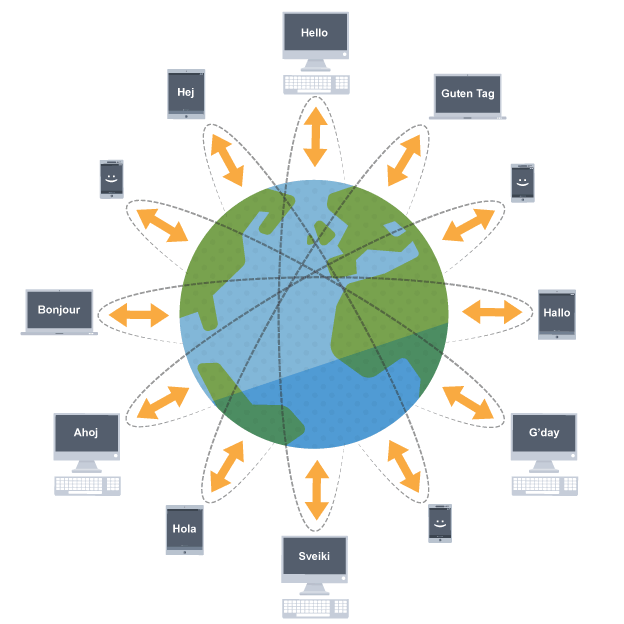
\includegraphics[width=11cm]{./net.png}
\footnotetext{All these pieces of hardware are usually addressed as \textbf{endpoints} as long as they have the ability to communicate effectively within a network}


Networking is crucial if you want to use your computer to communicate. Without it you couldn’t send an email, a text or an instant message and that would be so bad.

We use a huge network on a daily basis and this is called the internet. Around three billion people use the internet to share data, news and resources, amongst many other things.
\subsection{guided wiring}
Is quicker than unguided, it consists in physical wires. Optic Fiber is on the top of this list but can't be twisted. You can install a optic cable for a much longer distance and you won't get the same troubles you would get with copper cables for example

\subsection{unguided wiring}
This is Wi-Fi essentially. You can have a 2.5Ghz signal to reach longer distance but won't be nicely matched with a 5Ghz device

\section{LAN vs WAN}

LAN, which stands for local area network, and WAN, which stands for wide area network, are two types of networks that allow connection between computers. As the naming conventions suggest, LANs are for smaller, more localized networking — in a home, business, school, etc. — while WANs cover larger areas, such as cities, and even allow computers in different nations to connect. LANs are typically faster and more secure than WANs, but WANs enable more widespread connectivity

\clearpage



\section{IEEE 802.3}

IEEE 802.3 is a set of standards and protocols that define Ethernet-based networks. Ethernet technologies are primarily used in LANs, though they can also be used in WANs as well. IEEE 802.3 defines the physical layer and the medium access control (MAC) sub-layer of the data link layer for wired Ethernet networks.

\subesction{IEEE 802.3 Popular Versions}
There are a number of versions of IEEE 802.3 protocol. The most popular ones are.

\begin{itemize}
\item{IEEE 802.3: This was the original standard given for 10BASE-5. It used a thick single coaxial cable into which a connection can be tapped by drilling into the cable to the core. Here, 10 is the maximum throughput, i.e. 10 Mbps, BASE denoted use of baseband transmission, and 5 refers to the maximum segment length of 500m}
\item{IEEE 802.3a: This gave the standard for thin coax (10BASE-2), which is a thinner variety where the segments of coaxial cables are connected by BNC connectors. The 2 refers to the maximum segment length of about 200m (185m to be precise)}
\item{IEEE 802.3i: This gave the standard for twisted pair (10BASE-T) that uses unshielded twisted pair (UTP) copper wires as physical layer medium. The further variations were given by IEEE 802.3u for 100BASE-TX, 100BASE-T4 and 100BASE-FX}
\item{IEEE 802.3j: This gave the standard for Ethernet over Fiber (10BASE-F) that uses fiber optic cables as medium of transmission}
\end{itemize}
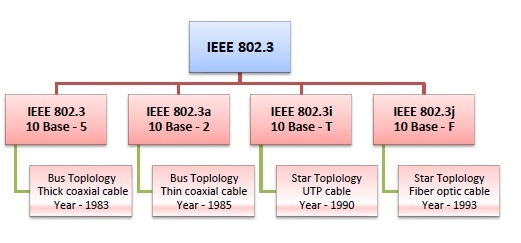
\includegraphics[width=15cm]{./ieee_802.jpg}

\clearpage
\printindex

\end{document}
